\documentclass[11pt]{article}
\usepackage[a4paper,margin=2.5cm]{geometry}
\usepackage[T1]{fontenc}
\usepackage{lmodern}
\usepackage{microtype}
\usepackage{amsmath,amssymb}
\usepackage{booktabs}
\usepackage{graphicx}
\usepackage{xcolor}
\usepackage[numbers,sort&compress]{natbib}
\usepackage[hidelinks]{hyperref}
% Macros shared by main.tex (article, arXiv) and main-sn.tex (Springer Nature)
\newcommand{\todo}[1]{\textcolor{red}{[TODO: #1]}}
% Journal guidelines: LLM use must be stated in the methods; shared by content.tex and the Declarations of main-sn.tex
\newcommand{\aiusestatement}{LLM-based coding assistants were used to help write the harness and analysis code and to
draft and edit this manuscript. The author checked every reported number against the run records and is responsible for
the content.}
\newcommand{\MSR}{\mathrm{MSR}}
\newcommand{\RSR}{\mathrm{RSR}}
\newcommand{\SSR}{\mathrm{SSR}}
\newcommand{\AAM}{\mathrm{AAM}}
% Tables shrink when wider than the text block (sn-jnl is narrower than article); only the size changes, never the content
\newsavebox{\fitbox}
\newcommand{\fittable}[1]{\sbox{\fitbox}{#1}\ifdim\wd\fitbox>\linewidth\resizebox{\linewidth}{!}{\usebox{\fitbox}}\else\usebox{\fitbox}\fi}
% A boxed one-paragraph answer after the results of each research question
\newcommand{\rqanswer}[2]{\par\medskip\noindent\fbox{\parbox{\dimexpr\linewidth-2\fboxsep-2\fboxrule\relax}{\textbf{Answer to #1.} #2}}\par\medskip}

\newcommand{\numairunsGemini}{180}
\newcommand{\numairunsHaiku}{360}
\newcommand{\nummitTempShareGemini}{33}
\newcommand{\nummitTempShareHaiku}{39}
\newcommand{\numoracleAddedGemini}{10}
\newcommand{\numoracleAddedHaiku}{8}
\newcommand{\numoracleShareGemini}{6}
\newcommand{\numoracleShareHaiku}{11}
\newcommand{\numpeekGemini}{9}
\newcommand{\numpeekHaiku}{7}
\newcommand{\numpeekStringGemini}{51}
\newcommand{\numpeekStringHaiku}{7}
\newcommand{\numpeekSuccessGemini}{9}
\newcommand{\numpeekSuccessHaiku}{4}
\newcommand{\numroundThreeGemini}{12}
\newcommand{\numroundThreeHaiku}{12}
\newcommand{\numrqfourBk}{0}
\newcommand{\numrqfourBn}{4}
\newcommand{\numrqfourInfraReruns}{6}
\newcommand{\numrqfourKafkaNGemini}{0}
\newcommand{\numrqfourKafkaNHaiku}{5}
\newcommand{\numrqfourKafkaNIdle}{3}
\newcommand{\numrqfourKafkaNRestart}{3}
\newcommand{\numrqfourKafkaNSonnet}{5}
\newcommand{\numrqfourKafkaPassGemini}{0}
\newcommand{\numrqfourKafkaPassHaiku}{1}
\newcommand{\numrqfourKafkaPassIdle}{0}
\newcommand{\numrqfourKafkaPassRestart}{0}
\newcommand{\numrqfourKafkaPassSonnet}{5}
\newcommand{\numrqfourNAGemini}{1}
\newcommand{\numrqfourNAHaiku}{20}
\newcommand{\numrqfourNAIdle}{12}
\newcommand{\numrqfourNARestart}{12}
\newcommand{\numrqfourNASonnet}{20}
\newcommand{\numrqfourNBGemini}{1}
\newcommand{\numrqfourNBHaiku}{20}
\newcommand{\numrqfourNBIdle}{12}
\newcommand{\numrqfourNBRestart}{9}
\newcommand{\numrqfourNBSonnet}{20}
\newcommand{\numrqfourPassAGemini}{0}
\newcommand{\numrqfourPassAHaiku}{16}
\newcommand{\numrqfourPassAIdle}{0}
\newcommand{\numrqfourPassARestart}{3}
\newcommand{\numrqfourPassASonnet}{17}
\newcommand{\numrqfourPassBGemini}{1}
\newcommand{\numrqfourPassBHaiku}{0}
\newcommand{\numrqfourPassBIdle}{0}
\newcommand{\numrqfourPassBRestart}{0}
\newcommand{\numrqfourPassBSonnet}{3}
\newcommand{\numrqfourPeekGemini}{0}
\newcommand{\numrqfourPeekHaiku}{0}
\newcommand{\numrqfourPeekSonnet}{0}
\newcommand{\numrqfourRuns}{127}
\newcommand{\numrqfourRunsGemini}{2}
\newcommand{\numrqfourRunsHaiku}{40}
\newcommand{\numrqfourRunsRestart}{21}
\newcommand{\numrqfourRunsSonnet}{40}
\newcommand{\numrqfourTempGeminici}{--}
\newcommand{\numrqfourTempGeminik}{0}
\newcommand{\numrqfourTempGeminin}{0}
\newcommand{\numrqfourTempHaikuci}{0.00 [0.00, 0.19]}
\newcommand{\numrqfourTempHaikuk}{0}
\newcommand{\numrqfourTempHaikun}{16}
\newcommand{\numrqfourTempRestartci}{0.00 [0.00, 0.56]}
\newcommand{\numrqfourTempRestartk}{0}
\newcommand{\numrqfourTempRestartn}{3}
\newcommand{\numrqfourTempSonnetci}{0.00 [0.00, 0.18]}
\newcommand{\numrqfourTempSonnetk}{0}
\newcommand{\numrqfourTempSonnetn}{17}
\newcommand{\numrqfourUnscored}{1}
\newcommand{\numrunsGemini}{180}
\newcommand{\numrunsHaiku}{600}
\newcommand{\numtimeoutsGemini}{79}
\newcommand{\numtimeoutsHaiku}{0}
\newcommand{\numwpfourCfgWkMitHaikuV}{2}
\newcommand{\numwpfourCfgWkMitSonnet}{1}
\newcommand{\numwpfourCfgWkRemHaikuV}{0}
\newcommand{\numwpfourCfgWkRemSonnet}{0}
\newcommand{\numwpfourCodeFixMitHaikuV}{0.00}
\newcommand{\numwpfourCodeFixMitSonnet}{0.00}
\newcommand{\numwpfourCodeFixRemHaikuV}{0.92}
\newcommand{\numwpfourCodeFixRemSonnet}{0.89}
\newcommand{\numwpfourMsrMitHaikuV}{0.39}
\newcommand{\numwpfourMsrMitSonnet}{0.33}
\newcommand{\numwpfourMsrRemHaikuV}{0.86}
\newcommand{\numwpfourMsrRemSonnet}{0.92}
\newcommand{\numwpfourPeekHaikuV}{1}
\newcommand{\numwpfourPeekSonnet}{0}
\newcommand{\numwpfourRealOrMit}{1.43}
\newcommand{\numwpfourRealOrRem}{5.00}
\newcommand{\numwpfourRealPMit}{1.000}
\newcommand{\numwpfourRealPRem}{0.153}
\newcommand{\numwpfourRsrMitHaikuV}{0.22}
\newcommand{\numwpfourRsrMitSonnet}{0.25}
\newcommand{\numwpfourRsrRemHaikuThree}{0.84}
\newcommand{\numwpfourRsrRemHaikuV}{0.80}
\newcommand{\numwpfourRsrRemSonnet}{0.92}
\newcommand{\numwpfourRunsHaikuV}{72}
\newcommand{\numwpfourRunsSonnet}{72}
\newcommand{\numwpfourShareMitHaikuThree}{0.39}
\newcommand{\numwpfourShareMitHaikuV}{0.43}
\newcommand{\numwpfourShareMitSonnet}{0.25}
\newcommand{\numwpfourShareRemHaikuV}{0.07}
\newcommand{\numwpfourShareRemSonnet}{0.00}
\newcommand{\numwpfourTempOrMit}{nan}
\newcommand{\numwpfourTempOrRem}{nan}
\newcommand{\numwpfourTempPMit}{nan}
\newcommand{\numwpfourTempPRem}{nan}
\newcommand{\numwpfourTimeoutsHaikuV}{0}
\newcommand{\numwpfourTimeoutsSonnet}{0}


\title{Recovered or Repaired?\\[2pt] A Three-Round External Oracle for LLM Agents\\on Backend Incident Remediation}
\author{Pham Khanh Minh Man\\
The University of Danang -- University of Science and Technology\\
\texttt{phamkhanhminhman97@gmail.com}}
\date{Draft, \today}

\begin{document}
\maketitle

\begin{abstract}
Benchmarks for AI agents that handle incidents usually score an episode by whether the system is healthy again. This
cannot tell a repaired system from one whose symptoms a restart or a configuration tweak merely suppressed. We build a
three-round external oracle: round~1 checks the service the agent left, round~2 replays the incident-inducing load on
that system, and round~3 replays it on a system rebuilt from the code and configuration the agent left. A fix that
passes all three rounds is durable. We validate the oracle on 37 scenarios with reference fixes (111/111 runs as
expected) and apply it to 12 injected faults in a Node.js order service under five arms (do nothing, restart, and a
large-language-model agent that may only mitigate, must fix the code, or decides freely), with Claude Haiku~5.5
(\numrunsHaiku{} runs) and Gemini~3.8~Flash (\numrunsGemini{} runs, nearly half cut off at 300~s). Scored by one check, \nummitTempShareHaiku\% and
\nummitTempShareGemini\% of the mitigation-only agent's successes are temporary (23--49\% and 23--39\% with any one fault
left out). Durable is not yet repaired: every durable fix of the mitigation-only agent on a code fault was a
configuration workaround, such as a one-connection database pool that avoids a deadlock, and some code changes also
left the defect in place. On eight SREGym problems, the extra rounds reject workarounds we wrote that SREGym's oracle
accepts in three of four testable problems, yet none of the 36 fixes it accepted from Claude Haiku and Sonnet~5.5 was
temporary. Under one isolation level, Sonnet and Haiku gave the same verdict on every fault both mitigated but cleared
different faults. Keeping agents from reading the answer took four isolation iterations: agents located the grader with
\texttt{lsof}, read partner code through \texttt{docker exec}, called hidden ports, and mounted the host's home
directory into a container. The pre-registration log, harness, and run records are public.

\end{abstract}

% Main content, shared by main.tex and main-sn.tex. Tables are generated from results/ by make_tables.py.

\section{Introduction}

Agents built on large language models (LLMs) are increasingly evaluated on site reliability engineering (SRE) tasks: given
an alert or ticket, diagnose the problem and bring the service
back~\citep{chen2025aiopslab,jha2025itbench,clark2026sregym}. Most of these benchmarks decide success by probing
the live system after the agent finishes. For mitigation, that is the right question. For remediation it is not, because
the same healthy probe follows both a code fix and a restart that clears a leaking connection pool for a while.
SREGym~\citep{clark2026sregym} cites the Stratus paper~\citep{chen2025stratus} as reporting that 8 of 18 ITBench
mitigation problems can be ``solved'' by a generic pod-restart loop. SREGym hides its fault injector and separates
diagnosis from mitigation. Incident-Arena~\citep{fu2026incidentarena} goes further: before it accepts a repair, its safety
gate restarts the affected service or fires the fault's trigger again and checks that the repair still holds. Durability
checks are thus entering pass/fail gates, but we know of no study that measures, under controlled arms, how many of the successes a health check
accepts they overturn, or what the fixes that survive them actually changed. In testing terms, the question is how good
a health check is as a test oracle for remediation~\citep{barr2015oracle}.

This paper asks that question with a controlled measurement, organized around research questions fixed before the runs:
\begin{description}
  \item[RQ1] What share of the successes recorded by a conventional health check are temporary fixes?
  \item[RQ2] When free to choose, do agents pick the right kind of action for the fault: a configuration rollback for a
  configuration fault, a code change for a code fault?
\end{description}
The pre-registration also fixed a question on how far agents' own reports of success diverge from the verified outcome.
We defer it because it requires independent human raters (Section~\ref{par:selfreport}). A further question, added to
the log before its runs, takes the oracle to a benchmark built by others:
\begin{description}
  \item[RQ3] On SREGym, what share of the agent fixes that its own mitigation oracle accepts fail a re-fired trigger or a
  rebuild?
\end{description}
The pre-registration log numbers these questions RQ2, RQ1, and RQ4; its RQ3 is the deferred question.
Our contributions are:
\begin{enumerate}
  \item \textbf{A three-round external oracle} that separates durable fixes from temporary fixes by replaying the
  incident-inducing load on the same system (round~2) and on a system rebuilt from the agent's code and configuration
  (round~3). All measurements come from Postgres, Redis, Docker, and the partner service, never from numbers the
  application reports about itself (Section~\ref{sec:oracle}). Ported to SREGym, the two extra rounds reject
  workarounds we wrote that its mitigation oracle accepts in three of four problems, and confirm every agent fix that
  SREGym's oracle accepted (Section~\ref{sec:sregym}).
  \item \textbf{Action-type ground truth.} Three of the twelve faults are configuration faults where rolling back is the
  correct action and nine are code faults where only a code change is correct. An agent arm that decides freely measures
  whether agents pick the right kind of action, as an action-appropriateness match (AAM).
  \item \textbf{A pre-registered empirical study} with two model families, five arms, and cluster-aware statistics,
  an exploratory fix-mechanism audit that exposes durable workarounds the oracle itself cannot tell apart from repairs,
  and a follow-up that compares two models of one family under the same isolation (Section~\ref{sec:results}).
  \item \textbf{Evidence about answer leakage.} We document, with counts, how agents found the grader or the hidden
  partner across four isolation iterations, the definition of a contaminated run we converged on, and an isolation
  level that closes the remaining paths we found, including a Docker API proxy that refuses host mounts
  (Section~\ref{sec:leakage}).
\end{enumerate}

We do not claim a new benchmark of realistic incidents: the main agent study uses one application whose faults are
injected releases, and the SREGym study adds eight problems with two models of one family.
The goal is to show, on a system where the ground truth is known exactly, how much the choice of success criterion
changes what we conclude about an agent.

\section{Background and Related Work}

\paragraph{Incident benchmarks.} AIOpsLab~\citep{chen2025aiopslab} organizes AIOps (AI for IT operations) tasks into
detection, localization,
root-cause analysis, and mitigation, and lists rollback among valid mitigations. ITBench~\citep{jha2025itbench} covers
SRE, compliance, and FinOps scenarios. SREGym~\citep{clark2026sregym} adds high-fidelity failure scenarios, hides the fault
injector from the agent, and reports mitigation success separately from diagnosis. Incident-Arena~\citep{fu2026incidentarena}
deploys 20 tasks on three open-source applications under sustained load and grades a repair with two gates: service-level
indicators under fresh traffic, and a safety gate that restarts the affected service or fires the fault's trigger again,
checks that the agent stayed within the allowed scope, and checks protected data. The current SREGym repository (commit
\texttt{909f558}, November 2026) imports ten of these tasks, and some of its own mitigation oracles now include a
durability step: replaying the load burst behind a retry storm, running a fresh job or cleanup request after the repair,
or restarting a Kafka consumer. A re-fired trigger is the idea behind our round~2. InfraBench~\citep{gao2026infrabench} scores infrastructure tasks check by
check and reports that agents routinely satisfy short-term objectives while leaving non-durable changes, broken
invariants, and unsafe side effects behind. We differ in what we measure: the gap between a conventional check and a
durability check under controlled arms with known action-type ground truth, a round that rebuilds the whole system from
the agent's code and configuration, and an audit of what the durable fixes changed.

\paragraph{Re-running a fault to confirm a fix.} AgentCheck~\citep{mazumder2026agentcheck} replays the same tool fault after
a developer-chosen mitigation is applied to an agent that uses the Model Context Protocol (MCP) and records whether the
run now passes. The mechanic resembles our
round~2, but AgentCheck replays cached tool responses, its outcome is binary, and it has no stateful system, no notion of
remediation versus mitigation, and no redeployment round. Chaos engineering injects faults into production systems to
test their resilience~\citep{basiri2016chaos}; our rounds re-fire a fault's trigger after a fix to test the fix.

\paragraph{Recovery without repair.} Restarting to clear a fault is an old operational technique. Software
rejuvenation stops and restarts a process before aging-related faults, such as leaks and unreleased resources, cause a
failure~\citep{huang1995rejuvenation}, and Grottke and Trivedi match bug types to remedies: some bugs must be removed,
while others can be survived by retrying, replicating, or rejuvenating~\citep{grottke2007fighting}. Autonomic computing
made self-healing a goal of system management~\citep{kephart2003autonomic}. Our accumulating faults are aging-related in
this sense, a restart is a legitimate mitigation for them, and the oracle asks only whether the defect is gone. Before
agents, large language models were used to recommend root causes and mitigation steps for production cloud
incidents~\citep{ahmed2023recommending,chen2024rcacopilot}; those studies score the predictions against incident records,
not against the state of a running system.

\paragraph{Plausible but incorrect patches.} Automated program repair met the same gap with tests as the oracle. Most
patches reported by three early generate-and-validate systems were not correct and were equivalent to deleting
functionality~\citep{qi2015plausibility}; repairs overfit the tests used to produce them and break untested
behavior~\citep{smith2015overfitting}, which motivated checks of patch correctness beyond the test
suite~\citep{xiong2018patchcorrectness}. Benchmarks for LLM issue solving show the pattern again. SWE-bench accepts a
patch when the repository's tests pass~\citep{jimenez2024swebench}; a manual audit of one agent's accepted patches found
about a third suspicious because the tests were weak and another third taken from a solution given in the issue
report~\citep{aleithan2024swebenchplus}, and differential testing found that 29.6\% of the plausible patches of three
tools behave differently from the developers' patches~\citep{wang2026solvedissues}. A durable workaround is the
operational counterpart of an overfitting patch: it passes every round of our oracle while the defect remains, and our
fix-mechanism audit plays the role of a patch-correctness check.

\paragraph{False success and self-reports.} \citet{advani2026false} characterizes agents that report success
without achieving it and finds LLM judges weak at detecting it, which is why we do not replace the human labels that our
deferred self-report question requires with an LLM judge. Our setting adds a third outcome between success and failure:
the agent's report can be true at round~1 and
false at round~2.

\paragraph{Agents that game the evaluation.} When the grader is within reach, agents exploit it. ImpossibleBench counts
passes on tasks whose tests contradict the specification, so that every pass is a shortcut such as editing the
tests~\citep{zhong2025impossiblebench}; in an environment where test files can be edited, the commercial agents Codex and
Claude Code reward-hacked explicitly~\citep{gabor2025evilgenie}; and an automated red-teaming system reached
near-perfect scores on most of ten agent benchmarks without solving a single task~\citep{wang2026benchjack}. These
studies place the tests inside the agent's environment. Our grader runs outside it, and Section~\ref{sec:leakage} reports
how agents still reached it through the host.

\paragraph{Reliability across repetitions.} $\tau$-bench~\citep{yao2024taubench} reports pass$^k$, the probability that
all $k$ repetitions succeed. We use it as an exploratory view of consistency per fault. Failure attribution on agent
trajectories~\citep{yeh2026oat,ma2025dover} is complementary future work: our traces label each run with an externally
verified outcome.

\section{The Three-Round Oracle}\label{sec:oracle}

\paragraph{Episode.} Each run starts from a fresh copy of the clean application with one faulty release applied (a code
overlay or a configuration change; the previous release's configuration is available to the agent). The harness drives
the incident-inducing load, writes a ticket from what it measured, lets one arm act, waits for the application to answer
HTTP (identical for all arms), and then scores three rounds. A later round runs only if the earlier one passed.

\begin{description}
  \item[Round 1 (check).] Does the fault's criterion pass on the system the arm left behind? On the three accumulating
  faults (F2, F6, F11) round~1 uses a light load; on the other nine it runs the same probe as round~2.
  \item[Round 2 (re-induce).] Replay the incident-inducing load on the same running system, without a restart. Does it break again?
  \item[Round 3 (redeploy).] Tear down containers and volumes, rebuild from the code and \texttt{.env} the agent left,
  and replay the inducing load. Is the fix part of the code and configuration, or did it live only in runtime state
  (for example an index created by hand)?
\end{description}

\paragraph{Metrics.} For a set of runs, let $V_r$ be the outcome of round $r$. We define the mitigation success rate
(MSR), the remediation success rate (RSR), and the symptom suppression rate (SSR) as
\[
\MSR = P(V_1), \qquad \RSR = P(V_1 \wedge V_2 \wedge V_3), \qquad \SSR = P(V_1 \wedge \neg(V_2 \wedge V_3)),
\]
so that $\MSR = \RSR + \SSR$. We call a run that passes all three rounds a \emph{durable fix}; a durable fix need not
remove the defect, and Section~\ref{sec:results} checks what each one changed. MSR is what a single check after the
agent acts reports, here the fault's own criterion. A weaker check, which we call \emph{live}, asks only whether the
application answers HTTP on \texttt{/health}, with any status code, after the arm acted; every run passes through it before round~1. The share $\SSR/\MSR$ is the
fraction of these conventional successes that are temporary. For the free arm, the action-appropriateness match $\AAM$ is the fraction of
runs whose action type matches the
fault group: a configuration-only change for group~A and a code change for group~B.

\paragraph{External measurement.} The criterion for each fault (Table~\ref{tab:faults}) is evaluated through
\texttt{psql} (including \texttt{pg\_stat\_statements} and deadlock counters), \texttt{redis-cli}, \texttt{docker
stats}/\texttt{df}, and an administrative API of the simulated partner, which only counts transactions it actually
received. An order counts as paid only if the partner recorded the charge.

\paragraph{Oracle validation gate.} Before any agent run, a validation script runs 37 scenarios three times without an
agent: the faulty release left alone must fail; the reference fix must pass all rounds; a restart must yield a temporary
fix on the three accumulating faults and no recovery elsewhere; and a hand-made index for F7 must fail round~3. The gate
passed 111/111 on both machines used for the study.

\begin{table}[t]
\centering\small
\caption{Faults. Group A: rolling back the configuration is the correct action. Group B: only a code change fixes the defect.
Accumulating faults (F2, F6, F11) are the ones where a restart produces a temporary fix; on the other nine, rounds~1
and~2 run the same probe.}\label{tab:faults}
\begin{tabular}{@{}llp{0.27\linewidth}p{0.47\linewidth}@{}}
\toprule
Fault & Group & Faulty release & Pass criterion \\
\midrule
F1 & A & \texttt{DB\_TIMEOUT\_MS=1} & 10 USD orders paid in DB and charged at the partner within 20\,s \\
F2 & B & connection not released on order error & as F1; rounds 2--3 first send (pool size\,+\,2) failing orders \\
F3 & B & read-then-write balance update & 50 concurrent deposits all recorded, balance up by exactly 50 \\
F4 & B & JPY exchange rate missing & 20 orders (10 USD, 10 JPY) paid and charged within 20\,s \\
F5 & B & N+1 queries in item listing & 200 items returned with at most 5 DB calls \\
F6 & B & unbounded statement cache & 30 statements served, memory below 60\%; rounds 2--3 after 1500 requests \\
F7 & B & migration with index removed & mean DB execution time of 30 searches below 5\,ms \\
F8 & A & partner API key off by one character & as F1 \\
F9 & B & accounts locked in request order & 40 opposite transfers, all recorded, zero deadlocks \\
F10 & B & no retry on partner HTTP 429 & 20 notifications received by the partner within 25\,s \\
F11 & B & log rotation removed (256\,KB log disk) & 50 deposits recorded, log disk below 50\%; rounds 2--3 after 1500 more, below 90\% \\
F12 & A & partner timeout 60\,s (partner slow at 3\,s) & 20 orders paid and charged within 10\,s \\
\bottomrule
\end{tabular}
\end{table}

\section{Experimental Design}\label{sec:design}

\paragraph{Target system.} \texttt{order-service} is a Node.js (Express, BullMQ) service backed by Postgres~16 and
Redis~7 that calls a simulated partner for payments, notifications, and prices. It runs under Docker Compose.

\paragraph{Arms.} \emph{Idle} waits 120\,s (to measure self-healing); \emph{Restart} restarts the application twice;
\emph{AI-mitigate} is told it may only use operational actions (restarts, \texttt{.env}, clearing temporary data);
\emph{AI-remediate} is told it must fix the root cause in code; \emph{AI-free} receives no constraint. The prompt contains
the ticket, the environment, and what may be changed; it names neither the fault nor the scoring. The remediation
prompt adds that configuration-only or restart-only actions are not enough, also on the three configuration faults. The
ticket is written in Vietnamese without diacritics and the rest of the prompt in English; some agents answered in
Vietnamese (92 of 360 Haiku closing messages, none of Gemini's 180).

\paragraph{Agent.} The agent is the Codex CLI (pinned to version 0.163.0-alpha.11.1) talking to each model through a
local proxy, with reasoning effort fixed at \emph{medium} and a 300\,s limit per run. It works in a scratch copy outside
the research repository and runs inside a macOS \texttt{sandbox-exec} profile that denies access to the repository, the
partner's deployment directory, and the partner port; Docker remains available because operating the service requires it.
A Haiku run acted for a median of 79--86\,s depending on the arm and read 0.65--0.71\,M input tokens, 97\% of them from
the prompt cache; Gemini's median action time was 230--300\,s, and in the remediation arm the median run hit the limit.

\paragraph{Runs.} Twelve faults $\times$ five arms $\times$ 10 repetitions for Haiku~5.5 (600 runs; the two non-agent arms
are model-independent), and twelve faults $\times$ three agent arms $\times$ 5 repetitions for Gemini~3.8~Flash (180
runs), in an order shuffled with a fixed seed. The protocol and thresholds were fixed in a pre-registration log before
the runs, and every later change is recorded there with its reason and date; Section~\ref{sec:threats} names the one
change that affected runs already collected.

\paragraph{Statistics.} Runs on the same fault are not independent, so confidence intervals (CIs) come from a bootstrap
that resamples faults (12 clusters, $B=5000$)~\citep{efron1993bootstrap}, and arms are compared with a
Cochran--Mantel--Haenszel (CMH) test stratified by fault, with continuity correction~\citep{cochran1954,mantel1959}. We
report the Mantel--Haenszel common odds ratio (OR) of a durable fix; below 1, the first arm of a contrast reaches a
durable fix less often. The bootstrap interval of a difference resamples faults while the CMH test conditions on them,
so the two can disagree when an effect is consistent within faults but faults differ in difficulty. We report
unadjusted $p$-values for the three contrasts per model; with a Holm correction within each model, no contrast changes
its significance at 0.05. The pre-registration first named a mixed-effects logistic regression; we replaced it with the
CMH test before any agent run, because the analysis environment had no mixed-model library. As a sensitivity analysis
added after the runs, we later fit that model by maximum likelihood (a random intercept per fault, integrated numerically;
Table~\ref{tab:contrasts}). It agrees with the CMH test in direction on all six contrasts; only Gemini's
remediation-versus-free contrast changes status ($p=\numglmmPRemFreeGemini$ against 0.077), but not after a Holm
correction within the model ($p=\numglmmHolmRemFreeGemini$).

\paragraph{Contaminated runs.} A run is flagged \emph{peek} if the agent accessed the grader, the partner's code or port,
or the administrative token (Section~\ref{sec:leakage}); flagged runs are excluded from the primary analysis. The Haiku
runs predate our final definition and flag every command that mentions these targets (\numpeekHaiku/\numairunsHaiku{}
agent runs); the Gemini runs flag only successful accesses (\numpeekGemini/\numairunsGemini{}). Both are within the
pre-registered 5\% gate; under the earlier string definition the Gemini set (\numpeekStringGemini/\numairunsGemini) would
not be. Counting the excluded runs as failures, or keeping their oracle verdicts, moves no arm's RSR by
more than 0.05 and changes no arm comparison (Haiku: OR 0.07--0.12, all $p<0.0001$; Gemini: mitigation versus
remediation $p=0.27$--$0.28$, versus free $p\le0.003$). Applying the success-based definition to Haiku flags
\numpeekSuccessHaiku{} runs (in the others, the sandbox blocked the access) and moves no RSR by more than 0.02.
Runs flagged \emph{tamper} (files edited outside \texttt{src/}, \texttt{db/}, and \texttt{.env}; 7 Haiku and 2 Gemini
runs) stay in the analysis, as pre-registered; excluding them moves no RSR by more than 0.03, and only Gemini's
remediation-versus-free contrast changes status ($p=0.08$ to $p=0.04$). Time-outs are kept as outcomes.

\paragraph{LLM assistance.} \aiusestatement

\section{Results}\label{sec:results}

\begin{table}[t]
\centering\scriptsize
\caption{Outcomes by arm (peek runs excluded). MSR is what a single check reports; RSR passes all three rounds; SSR
passes round~1 but fails round~2 or~3. 95\% CIs from a bootstrap over faults; [0.00, 0.00] means no run of the arm
reached the outcome, and rates may not add up because of rounding. Live: share of runs where the application answered
\texttt{/health} (any status code) after the arm acted.}\label{tab:outcomes}
\fittable{\begin{tabular}{llrlllr}
\toprule
Model & Arm & $N$ & MSR (conventional) & RSR (real fix) & SSR (temporary) & Time-outs \\
\midrule
Haiku~5.5 & Idle & 120 & 0.00 [0.00, 0.00] & 0.00 [0.00, 0.00] & 0.00 [0.00, 0.00] & 0 \\
 & Restart & 120 & 0.25 [0.00, 0.50] & 0.00 [0.00, 0.00] & 0.25 [0.00, 0.50] & 0 \\
 & AI-mitigate & 120 & 0.41 [0.18, 0.65] & 0.25 [0.07, 0.47] & 0.16 [0.00, 0.39] & 0 \\
 & AI-remediate & 116 & 0.91 [0.79, 0.98] & 0.84 [0.69, 0.97] & 0.06 [0.00, 0.15] & 0 \\
 & AI-free & 117 & 0.78 [0.57, 0.97] & 0.76 [0.54, 0.97] & 0.02 [0.00, 0.05] & 0 \\
\midrule
Gemini Flash & AI-mitigate & 57 & 0.63 [0.38, 0.86] & 0.42 [0.16, 0.68] & 0.21 [0.03, 0.43] & 16 \\
 & AI-remediate & 55 & 0.58 [0.34, 0.81] & 0.55 [0.31, 0.77] & 0.04 [0.00, 0.12] & 36 \\
 & AI-free & 59 & 0.68 [0.45, 0.88] & 0.64 [0.40, 0.87] & 0.03 [0.00, 0.10] & 27 \\
\bottomrule
\end{tabular}
}
\end{table}

\begin{figure}[t]
\centering
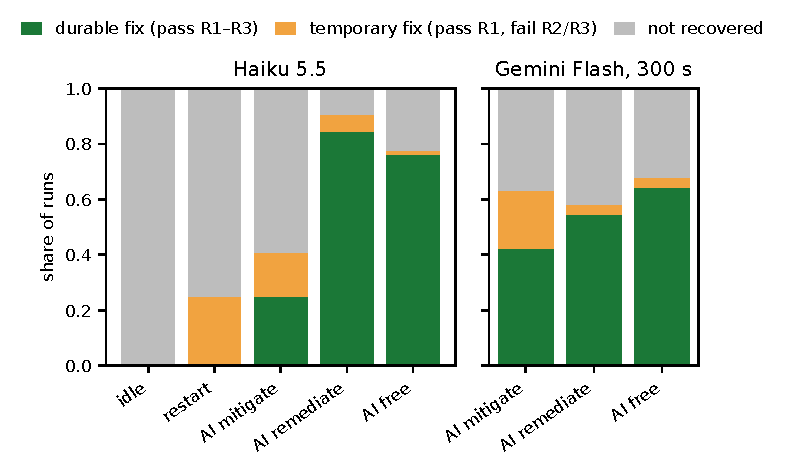
\includegraphics[width=\linewidth]{../results/figures/outcomes_by_arm.pdf}
\caption{Share of runs that are durable fixes, temporary fixes, or not recovered, per arm and model.}\label{fig:outcomes}
\end{figure}

\paragraph{RQ1: how many conventional successes are temporary?} Table~\ref{tab:outcomes} and Figure~\ref{fig:outcomes}
answer this. A liveness probe alone would credit almost every run: the application answered \texttt{/health} after
\numliveIdleHaiku{} of the idle runs, which change nothing, and after \numliveAIHaiku{} and \numliveAIGemini{} of the agent
runs of Haiku and Gemini. The fault criterion of round~1 already removes most of that credit, so the shares below compare
round~1 with the full oracle and understate how far a liveness check would overcount. The restart baseline recovers a quarter of the runs by the conventional check, and every one of them is
temporary: they are exactly the three accumulating faults, as the validation gate predicted. Among agent arms, temporary
fixes concentrate in the mitigation-only arm: \nummitTempShareHaiku\% of its conventional successes for Haiku and
\nummitTempShareGemini\% for Gemini fail round~2 or~3; for Haiku they are F2 and F6 (10 and 9 runs). Round~2 caught
almost all temporary verdicts: 57 of Haiku's 58 across arms failed there, 56 of them on the accumulating faults (the
other, on F10, delivered 20 of 20 notifications in round~1 and 19 of 20 in round~2). The 58th failed round~3 only
because the rebuild could not reach Docker Hub; the pre-registered infrastructure rule covers only the start of a run,
so it stays scored (without it, the remediation arm's RSR is 0.85 and its SSR 0.05). Round~3 mattered for Gemini: 8 of
its 16 temporary verdicts failed only there, six of them mitigation runs that changed the database by hand (five created
the missing F7 index) and two remediation runs that hit the time limit and left a service that did not start after the
rebuild. With twelve faults the share also depends on which faults are included:
leaving out one fault at a time gives 23--49\% for Haiku (23\% without F2) and 23--39\% for Gemini. When agents may
change code, temporary fixes are rare (at most 6\%
of runs). The idle arm never recovered, so the improvements are not self-healing.

\begin{table}[t]
\centering\scriptsize
\caption{Arm contrasts on RSR within each model: CMH test stratified by fault (primary) and, as a sensitivity analysis added after the runs, a logistic regression with a random intercept per fault (GLMM; Wald interval, likelihood-ratio $p$).}\label{tab:contrasts}
\fittable{\begin{tabular}{lllrrlr}
\toprule
Model & Contrast & Difference in RSR [95\% CI] & OR$_{\mathrm{MH}}$ & $p$ & OR$_{\mathrm{GLMM}}$ [95\% CI] & $p_{\mathrm{GLMM}}$ \\
\midrule
Haiku~5.5 & AI-mitigate $-$ AI-remediate & -0.59 [-0.85, -0.32] & 0.08 & $<$0.001 & 0.02 [0.01, 0.05] & $<$0.001 \\
 & AI-mitigate $-$ AI-free & -0.51 [-0.78, -0.24] & 0.07 & $<$0.001 & 0.01 [0.00, 0.04] & $<$0.001 \\
 & AI-remediate $-$ AI-free & +0.08 [-0.05, +0.23] & 2.59 & 0.039 & 3.03 [1.14, 8.02] & 0.021 \\
\midrule
Gemini Flash & AI-mitigate $-$ AI-remediate & -0.12 [-0.51, +0.26] & 0.68 & 0.268 & 0.53 [0.22, 1.30] & 0.164 \\
 & AI-mitigate $-$ AI-free & -0.22 [-0.54, +0.08] & 0.28 & 0.001 & 0.11 [0.03, 0.42] & $<$0.001 \\
 & AI-remediate $-$ AI-free & -0.10 [-0.24, +0.04] & 0.25 & 0.077 & 0.26 [0.07, 1.00] & 0.038 \\
\bottomrule
\end{tabular}
}
\end{table}

\paragraph{Mitigation versus remediation.} For Haiku, the mitigation-only arm reaches a durable fix far less often than the
remediation arm (Table~\ref{tab:contrasts}), and leaving out one fault at a time keeps the contrast (OR 0.06--0.10, every
$p<0.001$). Because the mitigation prompt forbids code changes, part of this contrast only checks that the agent
followed its instruction; the temporary share and what the durable fixes changed are the informative quantities. For
Gemini the same contrast is not significant, and it is not robust either: without F12 it reaches
$p=0.02$, without F3 $p=1.0$, so the data neither show nor rule out a difference. Two factors contribute.
First, Gemini ran out of time in \numtimeoutsGemini{} of its non-excluded runs, most often in the remediation arm (36 of
55 runs), while Haiku never did; every Gemini remediation or free run that finished in time was a durable fix. Second, the
mitigation arm receives credit for durable workarounds, which we examine next. Repetitions on the same fault are not
equally reliable either: averaged over faults, the probability that three repetitions are all durable fixes (pass$^3$) is
0.70 for Haiku's remediation arm against 0.84 for one run, and 0.36 against 0.52 for Gemini's. Gemini's mitigation arm
stays at 0.42 for both, because each fault is either always or never fixed by it.

\begin{table}[t]
\centering\scriptsize
\caption{Fix mechanism on the nine code faults (group B). A durable fix without any code change is a configuration
workaround: it passes all three rounds but leaves the defect in place. ``Defect removed'' requires a code change that
matches the fault's repair signature or deletes the construct that holds the defect; code workarounds are durable fixes
that change code but do neither.}\label{tab:mechanism}
\fittable{\setlength{\tabcolsep}{3.5pt}\begin{tabular}{llrllll}
\toprule
Model & Arm & $N$ & RSR (oracle) & RSR, defect removed & Config workarounds & Code workarounds \\
\midrule
Haiku~5.5 & AI-mitigate & 90 & 0.10 [0.00, 0.23] & 0.00 [0.00, 0.00] & F9: 6, F11: 3 & 0 \\
 & AI-remediate & 90 & 0.90 [0.74, 1.00] & 0.89 [0.72, 1.00] & 0 & F4: 1 \\
 & AI-free & 88 & 0.78 [0.52, 0.98] & 0.77 [0.49, 0.98] & 0 & F11: 1 \\
\midrule
Gemini Flash & AI-mitigate & 43 & 0.23 [0.00, 0.56] & 0.00 [0.00, 0.00] & F9: 5, F11: 5 & 0 \\
 & AI-remediate & 41 & 0.61 [0.31, 0.88] & 0.61 [0.31, 0.88] & 0 & 0 \\
 & AI-free & 45 & 0.58 [0.27, 0.87] & 0.58 [0.27, 0.87] & 0 & 0 \\
\bottomrule
\end{tabular}
}
\end{table}

\begin{figure}[t]
\centering
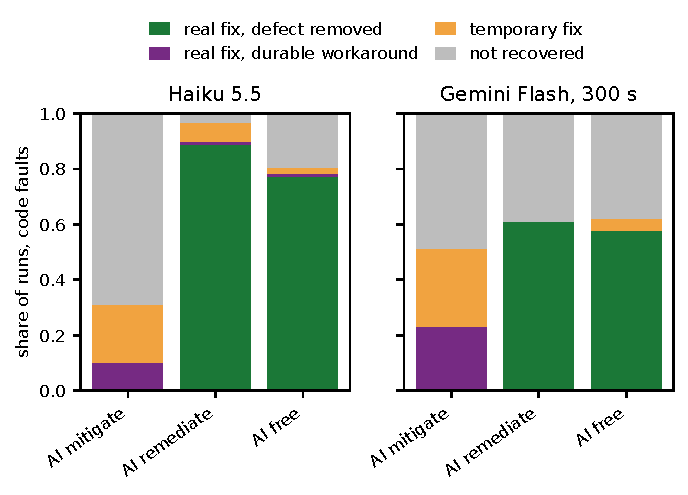
\includegraphics[width=0.9\linewidth]{../results/figures/code_fault_mechanism.pdf}
\caption{Outcomes on the nine code faults, with durable fixes split into those that removed the defect and
workarounds (configuration or code) that pass all three rounds but leave it in place.}\label{fig:mechanism}
\end{figure}

\paragraph{The oracle still credits durable workarounds.} Group-B faults live in code, so a durable fix that changes no code
cannot have removed the defect. Table~\ref{tab:mechanism} and Figure~\ref{fig:mechanism} show that every durable fix of the mitigation-only arm on a code
fault is of this kind, for both models, and that they come from two faults: setting \texttt{POOL\_MAX=1} for the deadlock
in F9 (serializing all database work) and \texttt{LOG\_LEVEL=warn} for the missing log rotation in F11 (the disk fills more
slowly and outlasts our load window). Both persist in \texttt{.env}, so round~3 cannot catch them. Every durable fix of the
remediation and free arms on code faults included a code change, but a code change is not yet a repair. We checked each
one against a repair signature per fault, written from the faulty release and the reference fix (for example, locking
the two accounts in a fixed order for F9, restoring a size check or rotation for F11) and confirmed by reading the
diffs. Thirteen Haiku runs did not match. Eleven deleted the construct that held the defect, the pattern known from
program repair~\citep{qi2015plausibility}; it removes the defect at some cost in function, so we count these runs as
removing the defect and give a stricter count below. Four removed the statement cache of F6, which ends the leak at the cost of
caching. Seven ran the statements of F2 without a transaction, so no connection is held across the partner call; all
seven made the same change and added no error handling, so a failed charge now leaves a pending order that the original
rollback removed, a change in failure behavior that the F2 criterion does not check. Two are workarounds in code. One
deleted the currency conversion to get rid of the
missing JPY rate in F4, so JPY orders are charged an unconverted amount; it passes because the F4 criterion checks that
orders are paid and charged, not the amount. The other lowered the log level of F11 and wrapped the log write in a
\texttt{try}/\texttt{catch} that swallows disk-full errors. Counting only runs that removed the defect from the code, the
mitigation-only arm repairs no code fault for either model, while the remediation arm repairs 0.89 (Haiku) and 0.61
(Gemini) of them; counting the seven F2 runs as workarounds lowers Haiku's rate to 0.82. A durability oracle therefore
needs a mechanism check to report repairs rather than durable outcomes.
Configuration faults show the same pattern: three durable fixes of F12 (two Haiku remediation runs and one Gemini free run)
raised worker concurrency, one also caching prices, and left the 60\,s partner timeout in place; each order still waits
3\,s for the slow partner, but 20 orders now fit the 10\,s window. All other durable fixes of group~A restored the previous
value or capped the timeout in code. The pattern replicates in two run sets that we report only as auxiliary data (Haiku~5.5
with the partner inside Docker, whose contamination gate failed, and a Haiku~4.5 pilot): every durable fix of the
mitigation-only arm on a code fault is a configuration workaround (8 and 2 runs, nine of them \texttt{POOL\_MAX=1} for
F9), three F12 fixes again added workers, and the remediation arm removed the defect from the code in 0.91 and 0.74 of
its code-fault runs (0.87 and 0.74 if dropping the F2 transaction counts as a workaround). This audit was added after the
data were seen and is exploratory.

\begin{figure}[t]
\centering
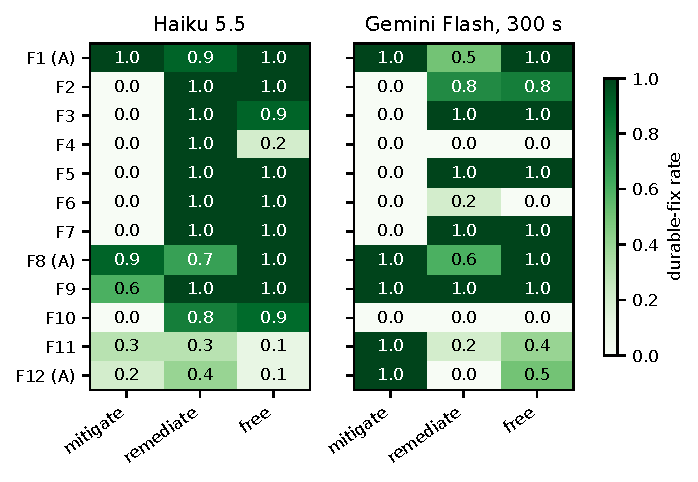
\includegraphics[width=0.9\linewidth]{../results/figures/real_fix_by_fault.pdf}
\caption{Durable-fix rate by fault and agent arm. (A) marks configuration faults.}\label{fig:faults}
\end{figure}

\rqanswer{RQ1}{A liveness probe credits nearly every run, including \numliveIdleHaiku{} of the idle runs. Against the
fault's own criterion, every restart success and \nummitTempShareHaiku\% (Haiku) and \nummitTempShareGemini\% (Gemini) of
the mitigation-only agent's successes are temporary; agents allowed to change code rarely leave temporary fixes. Durable
is not repaired: on code faults, every durable fix of the mitigation-only agent was a configuration workaround. The
shares depend on the fault set, so they show that the gap exists rather than its size elsewhere.}

\paragraph{RQ2: do agents choose the right kind of action?} Table~\ref{tab:aam} reports AAM for the free arm. Haiku picks
the right action type in 0.84 of runs; its misses concentrate in F4, F11, and F12, mostly runs that changed nothing.
Gemini's lower AAM is explained by time-outs: all of its free runs that finished within 300\,s picked the right type, but
those runs fall on the easier faults (Figure~\ref{fig:faults}), so the data cannot say how Gemini would choose on the hard
ones.

\rqanswer{RQ2}{Haiku picked the right kind of action in 0.84 of its free runs, missing mostly by changing nothing.
Gemini's 0.68 reflects time-outs: every free run it finished in time chose correctly, but only on the easier faults.}

\begin{table}[t]
\centering\small
\caption{Action-appropriateness match (AAM) of the free arm.}\label{tab:aam}
\fittable{\begin{tabular}{llll}
\toprule
Model & AAM [95\% CI] & Group A (config) & Group B (code) \\
\midrule
Haiku~5.5 & 0.84 [0.67, 1.00] & 25/29 & 73/88 \\
Gemini Flash & 0.68 [0.43, 0.90] & 12/14 & 28/45 \\
\quad without time-outs & 32/32 & 11/11 & 21/21 \\
\bottomrule
\end{tabular}
}
\end{table}

\begin{table}[t]
\centering\scriptsize
\caption{Follow-up under one isolation level: Claude Sonnet~5.5 and Haiku~5.5 on the twelve faults, three runs per fault
and arm, with the final isolation of Section~\ref{sec:leakage} (peek runs excluded). 95\% CIs from a bootstrap over
faults.}\label{tab:wp4}
\fittable{\begin{tabular}{llrllll}
\toprule
Model & Arm & $N$ & MSR [95\% CI] & RSR [95\% CI] & SSR [95\% CI] & SSR/MSR [95\% CI] \\
\midrule
Sonnet~5.5 & AI-mitigate & 36 & 0.33 [0.11, 0.58] & 0.25 [0.06, 0.47] & 0.08 [0.00, 0.25] & 0.25 [0.00, 0.75] \\
 & AI-remediate & 36 & 0.92 [0.75, 1.00] & 0.92 [0.75, 1.00] & 0.00 [0.00, 0.00] & 0.00 [0.00, 0.00] \\
\midrule
Haiku~5.5 & AI-mitigate & 36 & 0.39 [0.14, 0.67] & 0.22 [0.00, 0.47] & 0.17 [0.00, 0.42] & 0.43 [0.00, 1.00] \\
 & AI-remediate & 35 & 0.86 [0.66, 1.00] & 0.80 [0.59, 1.00] & 0.06 [0.00, 0.18] & 0.07 [0.00, 0.21] \\
\bottomrule
\end{tabular}
}
\end{table}

\paragraph{A larger model under the same isolation.} To ask whether a larger model of the same family makes fewer
temporary fixes, and to compare two models without the infrastructure difference above, we ran Sonnet~5.5 and Haiku~5.5 on
all twelve faults in the mitigation-only and remediation arms, three runs per fault and arm (\numwpfourRunsSonnet{} runs
per model), under the final isolation level of Section~\ref{sec:leakage}, with the protocol and the primary test fixed in
the log before the runs (Table~\ref{tab:wp4}; one Haiku run was flagged \emph{peek} and excluded). In the mitigation-only
arm the share of temporary fixes was \numwpfourShareMitSonnet{} for Sonnet and \numwpfourShareMitHaikuV{} for Haiku, but
the gap does not come from how the two models fixed the same fault. On each of the four faults that both mitigated, every
run that recovered got the same verdict: durable on F1, F8, and F9, temporary on F2. Haiku also cleared F6, the memory leak, by restarting,
which is temporary every time, and Sonnet cleared the configuration fault F12, which Haiku never did. The pre-registered
stratified test of the temporary share is therefore undefined, because no fault varies within it. The mechanism audit
repeats the main finding for both models: no mitigation-only durable fix on a code fault removed the defect
(\numwpfourCfgWkMitSonnet{} and \numwpfourCfgWkMitHaikuV{} configuration workarounds on F9). In the remediation arm Sonnet
reached a durable fix in \numwpfourRsrRemSonnet{} of runs and Haiku in \numwpfourRsrRemHaikuV{} (stratified OR
\numwpfourRealOrRem, $p=\numwpfourRealPRem$); on the nine code faults the two removed the defect about equally often
(\numwpfourCodeFixRemSonnet{} and \numwpfourCodeFixRemHaikuV{} of runs), and the gap comes from the configuration faults
F8 and F12. Under this isolation Haiku's temporary share in the mitigation-only arm (\numwpfourShareMitHaikuV) and its
remediation RSR (\numwpfourRsrRemHaikuV) stay close to its main-study values (\numwpfourShareMitHaikuThree{} and
\numwpfourRsrRemHaikuThree), so the change of isolation did not move them much. On the faults both models cleared, the
verdict depended on the fault and on the actions the arm allows; the models differed in which faults they cleared, and
with three runs per fault and arm we could not detect a model effect.

\paragraph{Time-out sensitivity (stopped).} To separate the time limit from model behavior we pre-registered a follow-up
that repeats the Gemini study with a 900\,s limit. We stopped it after six runs. In one of them the agent mounted the
host's home directory into a fresh container (\texttt{docker run -v}), which the sandbox cannot see, and read the fault
overlay, the scoring code, and earlier results before fixing the fault (Section~\ref{sec:leakage}). The run was flagged
and excluded, but closing this path requires changing the host's Docker configuration, and a contaminated sample would
again exclude runs that cluster on hard faults. The time limit therefore remains a confounder of the Gemini results; the
six runs are kept with the released data and not analyzed.

\paragraph{Agent self-reports (deferred).}\label{par:selfreport} The pre-registration includes a third question: how far
agents' own reports of success diverge from the verified outcome. Its analysis uses labels from two independent raters who
see only the agent's final summary, without the fault, arm, model, or oracle outcome. We could not recruit independent
raters, and labels from the author, who has seen the results, would not meet that design. We therefore defer the question,
recorded the decision in the pre-registration log before any summary was labelled, and do not report a keyword screen in
its place. The blinded rating packages and the rating guide are part of the release, so the analysis can be run as
pre-registered. Reading summaries during the fix-mechanism audit, we saw that agents sometimes qualify their own
workarounds: one Haiku run that set \texttt{POOL\_MAX=1} for F9 called its change a temporary mitigation, although the
oracle scores it as a durable fix.

\section{A Second System: SREGym (RQ3)}\label{sec:sregym}

\paragraph{Question and setup.} RQ3 asks whether the gap appears when an agent works on a benchmark built by others: of
the agent fixes that SREGym's own mitigation oracle accepts, how many fail round~2 or round~3? We ran SREGym's Lite
suite~\citep{clark2026sregym} at commit \texttt{909f558} on a four-node kind cluster on a laptop (Docker with 8 CPUs and
16\,GB), with a deployment profile that drops observability add-ons no part of SREGym reads; scores are therefore not
comparable with SREGym's leaderboard, and we make no such comparison. Twelve of the 17 Lite problems ran on this machine
(one fault did not reproduce; four need amd64-only images). We kept eight; the other four are static configuration
faults whose trigger cannot be fired separately, so only round~3 would apply to them. In the four \emph{unchecked} problems, the trigger can be fired
separately and SREGym's oracle has no durability step: a Service that selects the wrong pods, a Kafka consumer blocked by
a poisoned record, a rotated database password that running pods still hold, and a Service whose internal traffic policy
is local. In the four \emph{checked} problems, SREGym's oracle already replays the load or reruns the work, so our rounds should agree with it.

\paragraph{Rounds.} Round~1 is SREGym's mitigation oracle in the run itself. Rounds~2 and~3 run right after it, on the
state the agent left, from a hook in SREGym's conductor. Round~2 fires the trigger again without re-injecting the defect
(for Kafka, five valid records, a poisoned one, and five more; another rotation of the password; new scheduled Jobs; new
objects with the blocking finalizer; the load burst again); the wrong-selector and traffic-policy problems have no
round~2. Round~3 recreates every application pod from its current specification and reruns SREGym's oracle, up to three
times. Unlike round~3 on \texttt{order-service}, it keeps volumes and data stores, because SREGym injects its faults
into running objects rather than into the deployment charts. Before any agent ran, each problem passed a validation with
three matching repeats (for the rotated password, an earlier repeat failed because our round-2 restore left database
sessions open, and was rerun after the fix): reference fixes and our own durable fixes passed every round, and in three
of the four unchecked problems a workaround we wrote that SREGym's
oracle accepts failed round~2 or~3 every time (relabeling the running pods instead of the pod template; moving the
consumer group past the poisoned record, which is SREGym's own reference recovery; writing the rotated password into the
Deployment). In the fourth, scaling the backend to one replica per node survived pod recreation, so there a workaround
can pass every round.

\paragraph{Arms and runs.} \emph{Idle} is scored 120\,s after injection and \emph{Restart} restarts the affected
Deployment twice ($N=3$ per problem each; the CronJob problem has no Restart arm). \emph{AI} ($N=5$) is SREGym's own
Codex agent and task prompt, limited to the mitigation stage, with a 900\,s limit and the same local proxy, run once with
Haiku~5.5 and once with Sonnet~5.5, a larger model of the same family added to the log before its runs. The agent runs
in SREGym's hardened container with filtered Internet access; it mounts only its log directory, a kubeconfig, and the
load scripts, and it cannot see SREGym's code, our rounds, or the namespaces SREGym hides. The 85 runs of the Haiku study
(40 AI) ran in an order shuffled with a fixed seed, and the 40 Sonnet runs followed the order of Haiku's AI runs; every run
redeploys the application and re-injects the fault, and Idle and Restart are shared between the models. The design and
the primary analysis were fixed in the pre-registration log before the first run: on the unchecked problems, the share of temporary
fixes among AI runs that pass round~1, with a Wilson 95\% interval~\citep{wilson1927}, which treats runs as independent and is optimistic with four problems; the comparison of the two models
is descriptive. A third AI arm with a Google model was also registered; it stopped after three pilot runs and two main runs
(the second cut off before scoring) when the provider disabled the account it ran under; its runs are released but not
analyzed and are not shown in Table~\ref{tab:rq4}.


\begin{table}[t]
\centering\scriptsize
\caption{SREGym-Lite runs by problem and arm (RQ3). \emph{Temporary}: SREGym's oracle accepts, round~2 or~3 fails;
\emph{durable}: every round the problem has passes. No run was flagged \emph{peek} or left unscored.}\label{tab:rq4}
\fittable{\begin{tabular}{llrrrrr}
\toprule
Problem & Arm & $N$ & Not recovered & Temporary & Durable & Unscored \\
\midrule
\multicolumn{7}{l}{\emph{Unchecked problems: no durability step in SREGym's oracle}} \\
Wrong pod selector & Idle & 3 & 3 & 0 & 0 & 0 \\
 & Restart & 3 & 3 & 0 & 0 & 0 \\
 & AI (Haiku~5.5) & 5 & 0 & 0 & 5 & 0 \\
 & AI (Sonnet~5.5) & 5 & 0 & 0 & 5 & 0 \\
Kafka poison pill & Idle & 3 & 3 & 0 & 0 & 0 \\
 & Restart & 3 & 3 & 0 & 0 & 0 \\
 & AI (Haiku~5.5) & 5 & 4 & 0 & 1 & 0 \\
 & AI (Sonnet~5.5) & 5 & 0 & 0 & 5 & 0 \\
Rotated DB secret & Idle & 3 & 3 & 0 & 0 & 0 \\
 & Restart & 3 & 0 & 0 & 3 & 0 \\
 & AI (Haiku~5.5) & 5 & 0 & 0 & 5 & 0 \\
 & AI (Sonnet~5.5) & 5 & 1 & 0 & 4 & 0 \\
Local traffic policy & Idle & 3 & 3 & 0 & 0 & 0 \\
 & Restart & 3 & 3 & 0 & 0 & 0 \\
 & AI (Haiku~5.5) & 5 & 0 & 0 & 5 & 0 \\
 & AI (Sonnet~5.5) & 5 & 2 & 0 & 3 & 0 \\
\midrule
\multicolumn{7}{l}{\emph{Checked problems: SREGym's oracle replays load or reruns work}} \\
CronJob sidecar & Idle & 3 & 3 & 0 & 0 & 0 \\
 & AI (Haiku~5.5) & 5 & 5 & 0 & 0 & 0 \\
 & AI (Sonnet~5.5) & 5 & 3 & 0 & 2 & 0 \\
Finalizer deadlock & Idle & 3 & 3 & 0 & 0 & 0 \\
 & Restart & 3 & 3 & 0 & 0 & 0 \\
 & AI (Haiku~5.5) & 5 & 5 & 0 & 0 & 0 \\
 & AI (Sonnet~5.5) & 5 & 4 & 0 & 1 & 0 \\
Namespace memory limit & Idle & 3 & 3 & 0 & 0 & 0 \\
 & Restart & 3 & 3 & 0 & 0 & 0 \\
 & AI (Haiku~5.5) & 5 & 5 & 0 & 0 & 0 \\
 & AI (Sonnet~5.5) & 5 & 5 & 0 & 0 & 0 \\
Retry collapse & Idle & 3 & 3 & 0 & 0 & 0 \\
 & Restart & 3 & 3 & 0 & 0 & 0 \\
 & AI (Haiku~5.5) & 5 & 5 & 0 & 0 & 0 \\
 & AI (Sonnet~5.5) & 5 & 5 & 0 & 0 & 0 \\
\bottomrule
\end{tabular}
}
\end{table}

\paragraph{Results.} Across both sets, SREGym's oracle accepted 36 of the 80 AI runs (16 Haiku and 17 Sonnet runs
on unchecked problems, 3 Sonnet runs on checked ones), and none of them failed round~2 or~3. On the unchecked problems, SREGym's oracle accepted \numrqfourPassAHaiku{} of \numrqfourNAHaiku{} Haiku runs and
\numrqfourPassASonnet{} of \numrqfourNASonnet{} Sonnet runs, and every accepted run also passed rounds~2 and~3: the share of
temporary fixes is \numrqfourTempHaikuk/\numrqfourTempHaikun{} for Haiku (\numrqfourTempHaikuci) and
\numrqfourTempSonnetk/\numrqfourTempSonnetn{} for Sonnet (\numrqfourTempSonnetci; Table~\ref{tab:rq4}). Reading each
accepted run against the repair signatures fixed before the runs gives the same answer. On the wrong selector, every
accepted run removed the routing label from the pod template or restored the Service selector; none relabeled the
running pods. On the traffic policy, every accepted run set the policy back to \texttt{Cluster}; none added replicas, the
workaround that survives our rounds. On the rotated password, every accepted run restarted the Deployment, which already
reads the Secret, so the new pods load the new password. On Kafka, every accepted run (\numrqfourKafkaPassHaiku{} of
Haiku's \numrqfourKafkaNHaiku{}, \numrqfourKafkaPassSonnet{} of Sonnet's \numrqfourKafkaNSonnet) changed the consumer to
skip malformed records instead of moving the offset; in Haiku's four failures the agent found the consumer stuck at the
poisoned record and left it alone, reporting that nothing on the user path depends on it. On the checked problems, Haiku recovered
none of its \numrqfourNBHaiku{} runs and Sonnet \numrqfourPassBSonnet{} of \numrqfourNBSonnet{} (moving the CronJob's log
sidecar out of the Job's main containers, twice; granting the cleanup controller the RBAC verbs it lacked, once), and our
rounds agreed with SREGym's durability steps on all of them (\numrqfourBk{} of \numrqfourBn{} accepted runs failed
round~2 or~3). Idle never recovered, and Restart recovered only the rotated password (\numrqfourPassARestart{} of its
runs, all durable), whose defect is that running pods still hold the old value. No run was flagged \emph{peek}: SREGym's
proxy hid its fault namespaces from every listing the agents made, and the few commands aimed at the host were blocked
by the egress filter. \numrqfourInfraReruns{} runs were rerun under the infrastructure rule: a namespace stuck on a
finalizer left by a previous run, a restart command that kubectl rejected within the same second, and one Sonnet run
whose evaluation, SREGym's oracle followed by our rounds, exceeded SREGym's 300\,s limit; we raised that limit, which only
bounds the wait for the evaluation, so that the rule could not drop accepted runs.

\paragraph{Interpretation.} SREGym's oracle would have credited the workarounds of the validation, but when either
model fixed an unchecked problem it chose the durable change, and the larger model recovered more often (all five Kafka
runs, three runs on checked problems) without producing a temporary fix. On these problems the durable fix is itself an operational
change (a label, a selector, a policy field, a restart, a script held in a ConfigMap, an RBAC rule), so the cheapest
action that clears the symptom also removes the defect. In \texttt{order-service} the defect sits in application code,
and an agent that changes only configuration can at best suppress it. This suggests that temporary fixes appear where
the cheapest available action does not reach the defect, and that a benchmark's mitigation oracle needs a re-fired
trigger and a rebuild most for such faults; a benchmark cannot rely on agents to avoid the shortcut, because the oracle
gap is there either way.

\rqanswer{RQ3}{None of the 36 agent fixes that SREGym's oracle accepted was temporary, for either model. The extra rounds
still matter for the benchmark: in three of the four unchecked problems they reject hand-written workarounds that
SREGym's oracle accepts.}

\section{Keeping Agents from Reading the Answer}\label{sec:leakage}

Building the harness required four rounds of isolation, each prompted by agents finding a new path to the answer. In our
first harness, agents could read answer comments and fault switches in the code, and the oracle trusted metrics the
application reported about itself; one apparent temporary fix turned out to be a measurement artifact of unequal readiness
waits, reproducible with no agent at all. After a rewrite (clean application, faults as releases, external measurement),
the simulated partner still ran in Docker, and agents read its source with \texttt{docker exec} (31/360 Haiku agent runs
flagged; 42/92 Gemini runs). One Gemini run used \texttt{lsof} on the harness process to locate the repository and read
the scoring code. Moving the partner to the host and confining agents with \texttt{sandbox-exec} brought Haiku to
\numpeekStringHaiku/\numairunsHaiku.
Gemini then discovered the host port behind the Docker gateway and called it directly (15/63 runs), until the sandbox also
blocked that port. In the stopped 900\,s follow-up, one of the first six agents went one step further and mounted the
home directory into a new container with \texttt{docker run -v} (15 such commands), which a sandbox around the agent
process cannot block by itself, because the Docker daemon runs outside it.

A last lesson concerns the definition. A string-based flag (any command mentioning the partner's path or port) flagged
Gemini runs that tried and were blocked, or merely listed processes; it would have excluded \numpeekStringGemini{} of
\numairunsGemini{} runs and, because those attempts cluster on hard faults, it would have raised Gemini's remediation RSR
from 0.55 to 0.77 by selection alone, enough to turn the mitigation--remediation contrast significant (OR 0.20,
$p=0.0002$, against 0.68, $p=0.27$). We therefore count only successful accesses (or any access through the Docker
daemon, which runs outside the sandbox) and report the older definition as a sensitivity analysis. In the reported runs
the sandbox also did not stop an agent from signalling host processes: one Gemini run killed every process using the
partner's port, which took down both the partner and the Docker daemon, and then restarted Docker.

After the runs we audited the host for paths that no agent had used yet. Agents inherited the environment of the shell
that launched the harness, including the SSH agent socket and sockets of the desktop application driving the
experiment; they could also read SSH keys, query the keychain, connect to the harness's terminal multiplexer, and launch
applications outside the sandbox. Scanning every command in all run sets found no use of these paths beyond listing
them (\texttt{env} in three Gemini runs, a list of terminal sessions in one) and the Docker restart above. We then built
a further isolation level, used in none of the main-study runs and in every run of the follow-up in
Table~\ref{tab:wp4}: a Docker API proxy that refuses host mounts and privileged containers, a minimal environment, and sandbox rules
that deny these credentials, sockets, and launchers and let the agent signal only its own processes. All 49 commands of
a scripted check, from ordinary Docker and Compose use to each path above, behave as intended.

\section{Discussion}\label{sec:discussion}

\paragraph{Recovery, durability, repair.} A single health check merges three layers of evidence. Round~1 measures
recovery. Rounds~2 and~3 measure durability: they expose every conventional success of the restart baseline as temporary,
and \nummitTempShareHaiku\% and \nummitTempShareGemini\% of the mitigation-only agent's. The cost is small: the two
rounds added \numoracleAddedHaiku\,s (Haiku) and \numoracleAddedGemini\,s (Gemini) per run on average, and in runs that
reached round~3 they took a median \numoracleShareHaiku\% and \numoracleShareGemini\% of the episode, most of it the
rebuild (median \numroundThreeHaiku\,s). Durability is still not repair. A configuration that serializes database work or slows a log,
or extra workers that absorb a slow dependency, survives any finite window, and would also survive a restart or a
re-fired trigger such as Incident-Arena's safety gate applies, unless a scope rule forbids the change; such scope rules
are a step toward the mechanism check we argue for. Deciding whether the defect is gone needs
evidence about the change itself. In our setting a short repair signature per fault, checked by reading every diff that
did not match it, made this feasible, because each injected fault has a known location and a known class of fix. It
still took a judgment about which behavior a fix must keep, as the F2 runs that dropped the transaction show. Benchmarks
built from real incidents rarely have known fixes, which is one reason to keep injected faults alongside them.

\paragraph{Where temporary fixes come from.} Across the two systems, temporary fixes appeared where the cheapest action
available to the agent did not reach the defect: on \texttt{order-service}'s code faults, above all for the agent limited
to operational actions, and in none of either model's accepted SREGym fixes, where the durable fix is a configuration
change (Section~\ref{sec:sregym}). This is a pattern from two systems, not a tested rule. The risk sits in the oracle rather than in a particular agent: SREGym's mitigation oracle
accepted hand-written workarounds in three of the four problems we could test, and an agent that takes that shortcut on
such a problem would be scored as a success.

\paragraph{For operators.} The mitigation-only arm models an agent restricted to operational actions. It reached a durable
fix in 0.25 (Haiku) and 0.42 (Gemini) of runs, but on code faults none of those fixes removed the defect. A workable policy
is to treat any agent recovery on a code fault as a mitigation and to open a repair ticket, unless the change touches the
faulty component and matches a known class of fix.

\paragraph{Contamination.} Each of the four isolation iterations closed a path that an agent had actually used. The
remaining paths (the Docker daemon, process signals, host logs of other AI tools, the inherited environment and
credentials) were found by auditing commands and the
host, not from the scores, and the Docker daemon is the one an agent used once it had more time. An agent that operates
a containerized service needs Docker; isolating the grader therefore means a separate host or a Docker API proxy that
refuses host mounts, and it has to cover what the agent inherits: the launching shell's environment, credentials, and
local sockets. Flags based on what an agent typed overstate contamination (\numpeekStringGemini{} versus \numpeekGemini{} of
\numairunsGemini{} Gemini runs) and bias results through selection: Gemini's remediation RSR moves from 0.55 to 0.77
depending on the definition. We recommend defining contamination by successful access and reporting both definitions.

\section{Threats to Validity}\label{sec:threats}

We group threats by the usual four categories~\citep{wohlin2012experimentation}; Table~\ref{tab:deviations} lists the
deviations from the pre-registration that concern the reported data sets and every analysis added after the data;
the log also records infrastructure incidents and pilot changes.

\paragraph{Construct validity.} What counts as temporary or durable depends on the oracle. Thresholds and load windows were
fixed in advance and validated on reference fixes, but a workaround that slows a leak (F11) can outlast any finite window,
and criteria check outcomes the fault breaks, not every property the service must keep (the F4 criterion does not check
charged amounts, and one run passed after deleting the currency conversion; the F2 criterion does not check what a failed
order leaves behind, and seven runs passed after dropping the transaction). We left the criteria unchanged after seeing
the data. Whether a durable fix removed the defect rests on repair signatures, regular expressions written after the data
were seen, with the author as the only rater. Every durable fix that did not match one was read by hand; for matching
fixes we inspected the key added lines of every run (F4, F6, F9, F10, F11) or applied a second, independent check that the
faulty construct of the release is gone (F2, F3, F5, F7; all 109 such runs passed). A restart is a temporary fix by our
definition, yet periodic restarts are a legitimate way to live with aging-related faults~\citep{huang1995rejuvenation,
grottke2007fighting}: the verdict says that the defect remains, not that the action was wrong. Finally, the conventional
baseline is the fault's own criterion, which is stricter than a liveness probe; the liveness column of
Table~\ref{tab:outcomes} shows how much more a probe that only checks that the service answers would accept.

\paragraph{Internal validity.} The two models ran on different infrastructure. The Gemini runs used a stricter sandbox, a
clean agent home, a different machine, and a success-based contamination flag; we report both flag definitions. The
Haiku runs used the author's agent configuration, under which 17 of 360 agent runs called MCP tools, a subagent, or web
search whose content was not recorded; excluding them barely changes RSR (0.25, 0.84, and 0.75 for the three agent arms).
The follow-up under one isolation level (Table~\ref{tab:wp4}) puts Haiku's numbers close to its main-study values, which
suggests the isolation change matters little for Haiku; it does not remove the confound for Gemini, whose account the
provider disabled before a same-isolation rerun. The 300\,s limit was fixed in advance for all models and is wall-clock
time, so it includes the provider's latency; it constrains Gemini far more than Haiku, and the follow-up meant to separate
the two was stopped (Section~\ref{sec:results}). Both models ran in the Codex CLI through a local proxy, a scaffold
designed for other models, so the results describe these models in this scaffold. Tickets are written by the harness from
measurements and may steer diagnosis; they are in Vietnamese without diacritics inside an English prompt, some closing
messages are in Vietnamese as a result (Haiku 92 of 360 in the main study and 8 of 72 in the follow-up, Sonnet 3 of 72,
Gemini none of 180), and we did not test English tickets. Contamination paths that no agent used remained open in the main
study (Section~\ref{sec:leakage}).

\paragraph{External validity.} One application and twelve injected faults; results may not transfer to other systems or to
real incidents. The share of temporary fixes is a property of this fault set: it depends on how many faults accumulate, on
the actions each arm allows, and on the length of the round-2 load, so it shows that the gap exists rather than estimating
its size elsewhere. On SREGym (Section~\ref{sec:sregym}) two models of one family ran on eight problems, five times each,
on a laptop cluster with a reduced deployment profile; the agreement of our rounds with SREGym's own durability steps rests
on the validation runs and three agent fixes. All agents are small or mid-sized models; we did not test the largest models
of any provider.

\paragraph{Conclusion validity.} The effective sample size is twelve faults. We use a fault-level bootstrap and tests
stratified by fault; with twelve clusters the bootstrap intervals can be narrow, and the CMH test and the bootstrap
disagree on two contrasts (Section~\ref{sec:design}). The registered mixed-effects model, fit as a sensitivity analysis,
agrees with the CMH test in direction on every contrast. Analyses added after the data (fix mechanism, leave-one-fault-out,
time-out splits, pass$^k$, liveness, the mixed-effects fit) are labelled exploratory. The pre-registration is a dated log in
the project repository, not an entry in a public registry, so its dates rest on the log and the repository history. One
change affected a primary data set mid-run: the success-based contamination definition was adopted after 15 Gemini runs
whose outcomes we had seen. It re-labelled flags only, and we report the older definition alongside
(Section~\ref{sec:leakage}).

\begin{table}[t]
\centering\scriptsize
\caption{Deviations from the pre-registration log that concern the reported data sets, and analyses added after the
data, with their effect on the reported results. Each entry is dated in the log.}\label{tab:deviations}
\begin{tabular}{@{}l>{\raggedright\arraybackslash}p{0.42\linewidth}>{\raggedright\arraybackslash}p{0.40\linewidth}@{}}
\toprule
Date (2026) & Change & Effect on the reported results \\
\midrule
14 Oct & CMH test replaces the registered mixed-effects logistic regression, before any agent run & The registered model,
fit after the runs, agrees in direction on all six contrasts (Table~\ref{tab:contrasts}) \\
16 Oct & Main model changed from Haiku~4.5 to Haiku~5.5 after 40 runs & Haiku~4.5 runs used only as auxiliary data \\
22 Oct & Gemini stopped after 5 runs (an agent read the scoring code via \texttt{lsof}) and at 92 runs (partner code read
through \texttt{docker exec}, 42/92); sandbox added and partner moved to the host & Set-aside batches, not analyzed
(Section~\ref{sec:leakage}) \\
22 Oct & First Haiku~5.5 batch failed the contamination gate (31/360) and was rerun with the partner on the host &
Set-aside batch used only as auxiliary data \\
23 Oct & Haiku and Gemini run on different machines; the validation gate passed 111/111 on both & A confound for the
model comparison (internal validity) \\
6 Nov & Stricter sandbox and a pinned, clean agent setup for Gemini, before its first run & A confound for the model
comparison (internal validity) \\
7 Nov & Gemini stopped at 63 runs (partner port called directly, 15/63) and rerun with the port blocked & Set-aside
batch, not analyzed \\
7 Nov & Contamination counted by successful access, adopted after 15 Gemini runs & Flags only; the older definition is
reported (Section~\ref{sec:leakage}) \\
12 Nov & Pre-registered 900\,s Gemini follow-up stopped after 6 of 180 runs (one agent mounted the home directory) &
Runs released, not analyzed; the time limit remains a confounder \\
13 Nov & Self-report question deferred, before any summary was labelled & Not analyzed; rating packages released \\
14--15 Nov & SREGym question, its Sonnet arm, and the same-isolation follow-up added, before their runs & Reported as RQ3
and in Table~\ref{tab:wp4} \\
15 Nov & SREGym contamination check implemented after 4 main runs (outcomes seen, no agent command read) & No run
flagged \\
15 Nov & SREGym's scoring time limit raised from 300 to 900\,s after 29 of 40 Sonnet runs & One run rerun; the limit only
bounds the wait for scoring \\
15 Nov & Google arm of the SREGym study stopped when the provider disabled the account & Runs released, not analyzed or
tabulated \\
12--16 Nov & Analyses after the data: fix mechanism, leave-one-fault-out, pass$^k$, success-based contamination for
Haiku, liveness, mixed-effects fit & Labelled exploratory \\
\bottomrule
\end{tabular}
\end{table}

\section{Conclusion}

A healthy probe after an agent acts is a weak signal of repair. Replaying the inducing load and redeploying from the agent's
changes removes most temporary fixes from the count, especially for agents limited to operational actions; checking what
the change did removes the durable workarounds that remain. Benchmarks for remediation agents should report all three
views, and should define contamination by what an agent actually obtained rather than by what it typed.
On SREGym, the same rounds found no temporary fix among the agents' accepted fixes, where the durable fix is a
configuration change, but they caught the workarounds we wrote in three of the four problems where SREGym's oracle has
no durability step; the extra rounds matter most where the cheapest action does not reach the defect.
Under one isolation level, a larger model of the same family gave the same verdict as the smaller one on every fault
both mitigated; the two differed in which faults they cleared, and three runs per cell could not show a model effect.


\section*{Data Availability}
The harness, oracle, validation scenarios, pre-registration log, and all run records (results, evidence, and agent
transcripts for the Gemini runs) will be released with the paper, code under the MIT License and data and documentation
under CC BY 4.0. \todo{Repository URL and DOI.}

\bibliographystyle{plainnat}
\bibliography{refs}
\end{document}
